\documentclass{beamer}
\usepackage{graphicx}
\usepackage{multimedia}
\usetheme{metropolis}
\usepackage{multicol}
\usepackage{mathtools}
\usepackage[absolute,overlay]{textpos}
\setlength{\TPHorizModule}{\paperwidth}
\setlength{\TPVertModule}{\paperheight}
\mathtoolsset{showonlyrefs}
\title{MAE 259B Group 2 Progress Report}
\date{\url{https://github.com/kmxz/mae259b-project}}
\author{Siyuan Chen, Xiangzhou Kong, Long Chen}
\begin{document}
    \maketitle
    \begin{frame}{What we did - Starting point}
        \textbf{Start from the homework code}\\
	    Adapted from the MATLAB sample code, translated into Python, with minor changes and optimizations
        
        \textbf{Build utilities}\\
        Command line interface, 3D visualization tool, code snapshot tool, etc.
        
        \begin{center}
        	 \movie[width=4.0073cm,height=3.3927cm,showcontrols,poster,loop]{(Video: hw-render)}{res/hw-render.mp4}
        	 \hspace{2cm}
        	 \movie[width=4.0073cm,height=3.3927cm,showcontrols,poster,loop]{(Video: hw-nodes)}{res/hw-nodes.mp4} 
        \end{center}
    \end{frame}
    \begin{frame}{What we did - Performance optimization}
    	Profiling shows $90\%$ of time is spent on calculating $F$ and $J$
    	
    	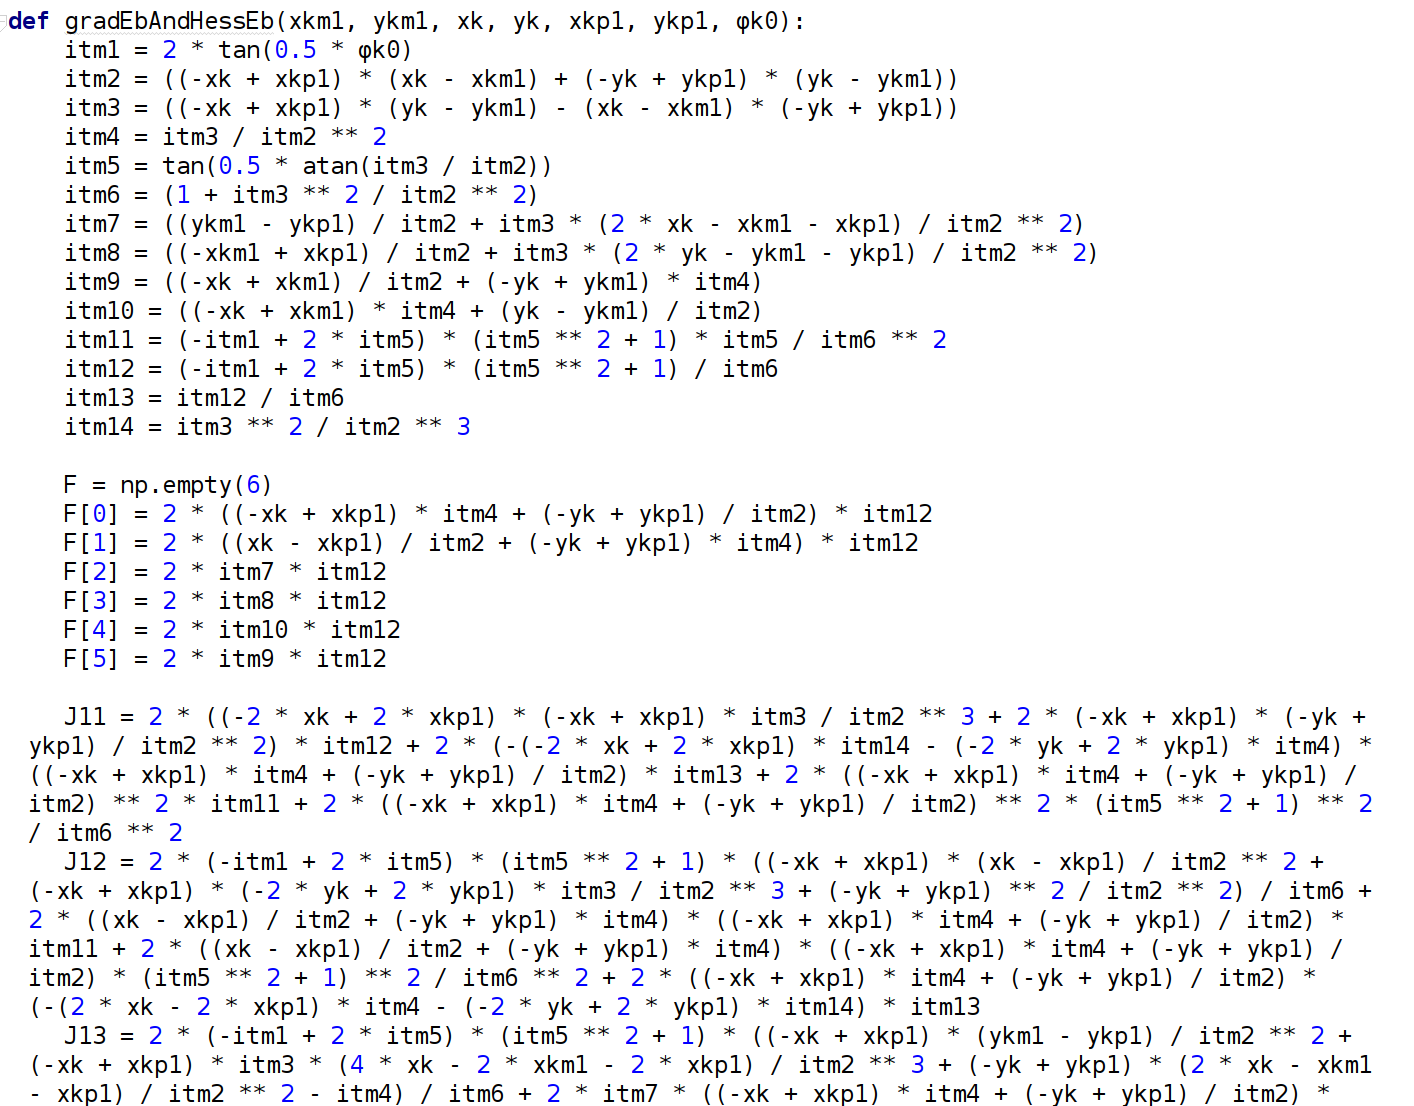
\includegraphics[width=0.9\textwidth]{res/getFb.png}
    	\begin{textblock}{0.3}[1,0](1,0.25)
		    \begin{center}
		    	\Large $30.6\,\mathrm s$\\$\Downarrow$\\$7.6\,\mathrm s$\\\bf 4x faster
		    \end{center}
    	\end{textblock}
	\end{frame}
	\begin{frame}{What we did - Initial curvature}
		When calculating bending energy, replace $(\phi_k)^2$ with $(\phi_k - \phi_{k0})^2$
		
		The formulas for calculating $F$ and $J$ need to be changed (do differentiation again)
		
		\begin{center}
			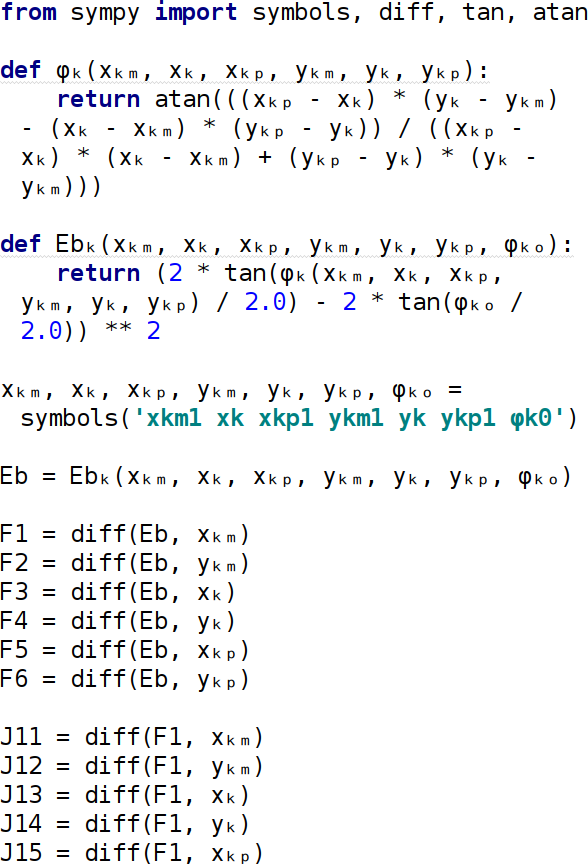
\includegraphics[width=0.6\textwidth]{res/diff.png}
		\end{center}
	\end{frame}
	\begin{frame}{What we did - Circular structure}
		\small
		Instead of $nv - 1$ edges, we have $nv$ edges.\\
		For bending, instead of $nv - 2$ components, we have $nv$ components.\\
		For stretching, instead of $nv - 1$ components, we have $nv$ components.
		
		When compositing the Jacobians, new components added to connect two ends together:
		
		\begin{center}
			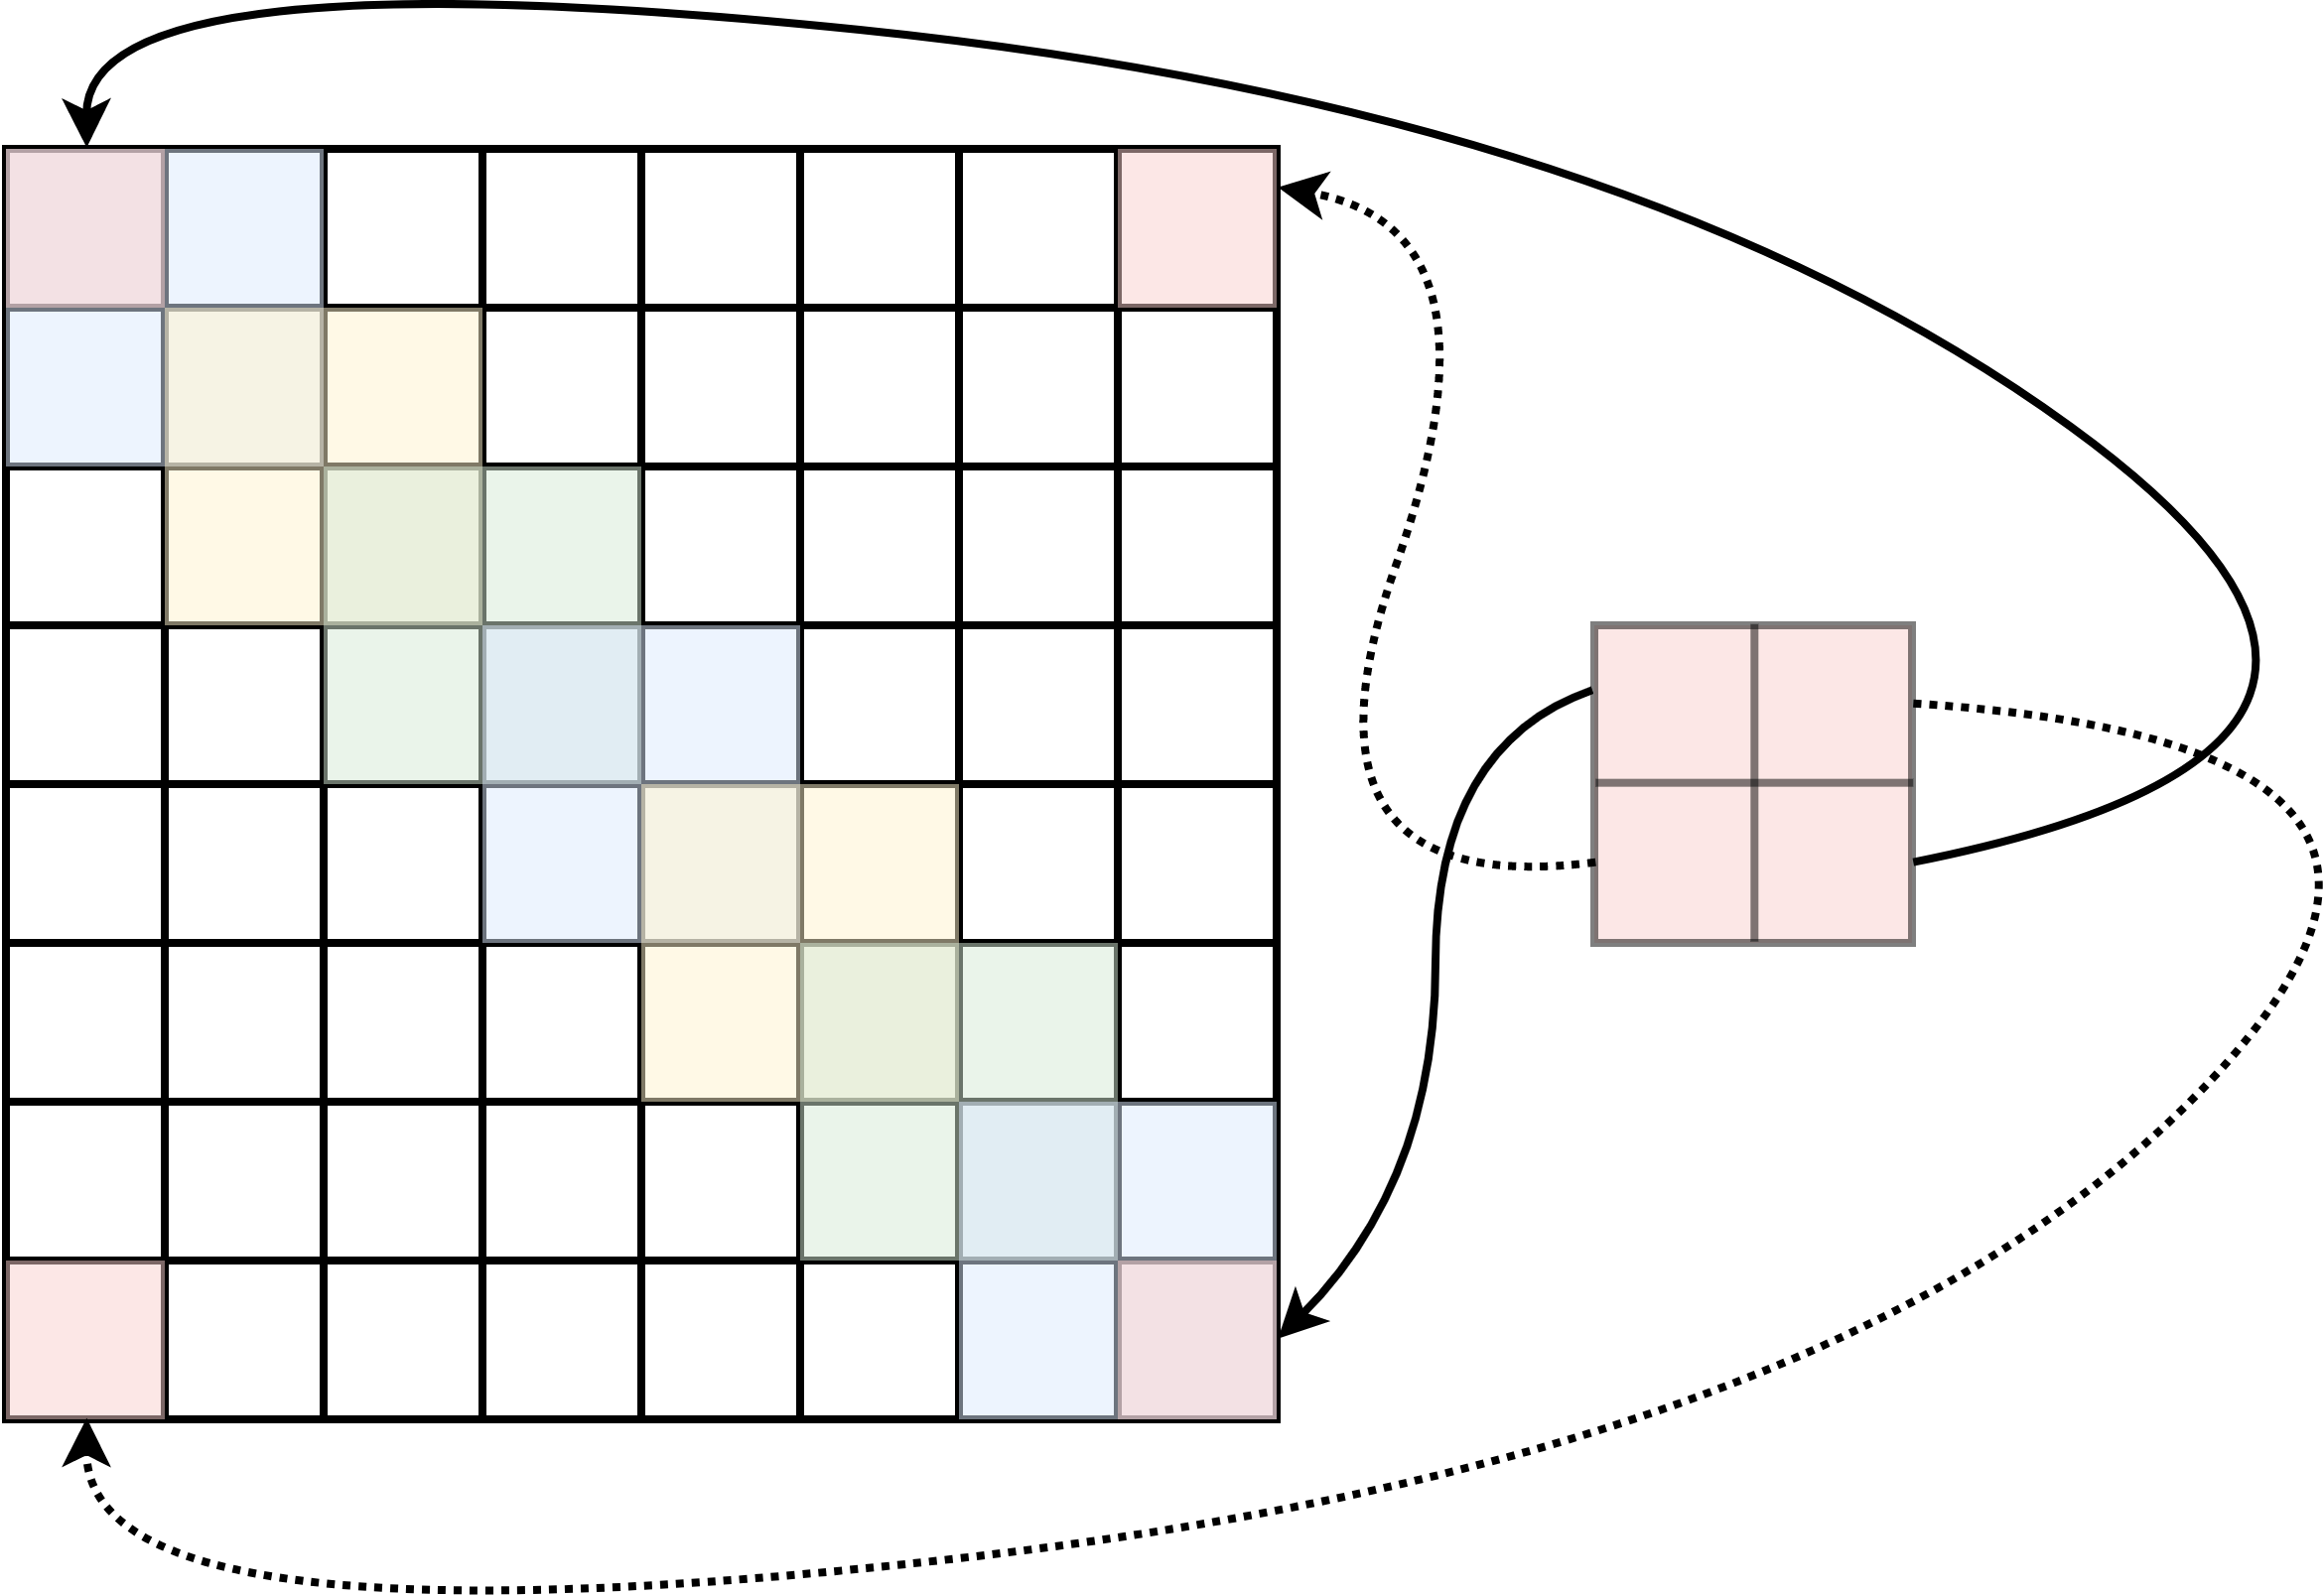
\includegraphics[width=0.6\textwidth]{res/composition.png}
		\end{center}
	\end{frame}
	\begin{frame}{What we did - Circular structure}
		Verify our code by running the ``hanging circle''
		
		\begin{tabular}{ccc}
			$Y = 10^6\,\mathrm{Pa}$ & $Y = 10^7\,\mathrm{Pa}$ & $Y = 10^8\,\mathrm{Pa}$\\
			\movie[width=3.09cm,height=3.11cm,showcontrols,poster,loop]{(Video: 1e6)}{res/1e6.mp4} & 
			\movie[width=3.09cm,height=3.11cm,showcontrols,poster,loop]{(Video: 1e7)}{res/1e7.mp4} & 
			\movie[width=3.09cm,height=3.11cm,showcontrols,poster,loop]{(Video: 1e8)}{res/1e8.mp4}
		\end{tabular}
	\end{frame}
	\begin{frame}{What we did - Inflation pressure}
		\begin{center}
			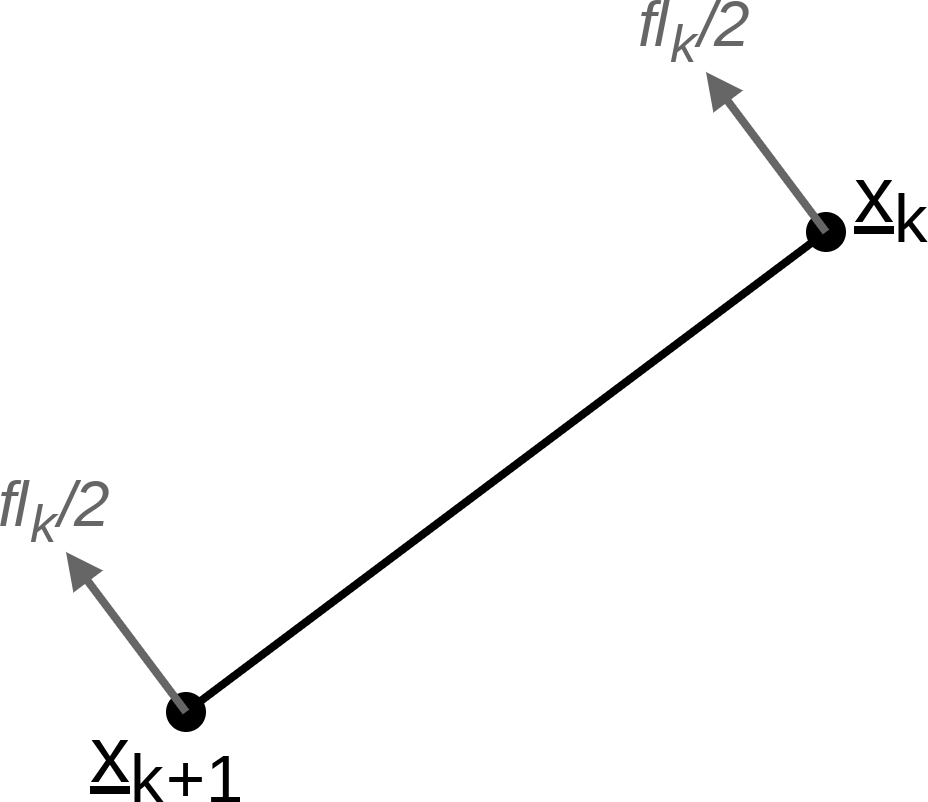
\includegraphics[width=0.4\textwidth]{res/inflation.png}
		\end{center}
	
		With $\underline x_k$ and $\underline x_{k+1}$, we can easily calculate force exerted on those two points. Taking derivatives on the forces, we have the corresponding Jabobian matrix. 
	\end{frame}
\end{document}